\section{Introduction and Background}
% (A short general text about the area of ai that your project belongs to.)
Chinese Checkers is a board game that can be played by two to six players.
Each player controls ten pegs that are placed in the corners of a
hexagonal star. The board has little holes in it where the pegs can be
placed. In each round of the game a player must move a peg in one of
two ways. A peg can be moved to one of the six holes next to it or, if
one of the holes is occupied by another peg, it can also ``jump'' over
that peg in a straight line (thereby traveling two holes over). The
player can jump over other pegs an unlimited number of times every
round, potentially moving a peg straight across the whole board. The
objective is to move all pegs to the opposite corner.
% Maybe it would be nice to add a few lines about the history of the game ?

\begin{figure}
\centering
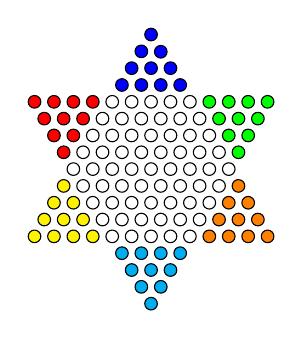
\begin{tikzpicture}
\filldraw [fill=blue] (0.000000,1.708957) circle (0.08);
\filldraw [fill=blue] (-0.123333,1.495337) circle (0.08);
\filldraw [fill=blue] (0.123333,1.490204) circle (0.08);
\filldraw [fill=blue] (-0.246667,1.281718) circle (0.08);
\filldraw [fill=blue] (0.000000,1.281718) circle (0.08);
\filldraw [fill=blue] (0.246667,1.281718) circle (0.08);
\filldraw [fill=blue] (-0.370000,1.068098) circle (0.08);
\filldraw [fill=blue] (-0.123333,1.068098) circle (0.08);
\filldraw [fill=blue] (0.123333,1.068098) circle (0.08);
\filldraw [fill=blue] (0.370000,1.068098) circle (0.08);
\filldraw [fill=red] (-1.480000,0.854478) circle (0.08);
\filldraw [fill=red] (-1.233333,0.854478) circle (0.08);
\filldraw [fill=red] (-0.986667,0.854478) circle (0.08);
\filldraw [fill=red] (-0.740000,0.854478) circle (0.08);
\filldraw [fill=white] (-0.493333,0.854478) circle (0.08);
\filldraw [fill=white] (-0.246667,0.854478) circle (0.08);
\filldraw [fill=white] (0.000000,0.854478) circle (0.08);
\filldraw [fill=white] (0.246667,0.854478) circle (0.08);
\filldraw [fill=white] (0.493333,0.854478) circle (0.08);
\filldraw [fill=green] (0.740000,0.854478) circle (0.08);
\filldraw [fill=green] (0.986667,0.854478) circle (0.08);
\filldraw [fill=green] (1.233333,0.854478) circle (0.08);
\filldraw [fill=green] (1.480000,0.854478) circle (0.08);
\filldraw [fill=red] (-1.356667,0.640859) circle (0.08);
\filldraw [fill=red] (-1.110000,0.640859) circle (0.08);
\filldraw [fill=red] (-0.863333,0.640859) circle (0.08);
\filldraw [fill=white] (-0.616667,0.640859) circle (0.08);
\filldraw [fill=white] (-0.370000,0.640859) circle (0.08);
\filldraw [fill=white] (-0.123333,0.640859) circle (0.08);
\filldraw [fill=white] (0.123333,0.640859) circle (0.08);
\filldraw [fill=white] (0.370000,0.640859) circle (0.08);
\filldraw [fill=white] (0.616667,0.640859) circle (0.08);
\filldraw [fill=green] (0.863333,0.640859) circle (0.08);
\filldraw [fill=green] (1.110000,0.640859) circle (0.08);
\filldraw [fill=green] (1.356667,0.640859) circle (0.08);
\filldraw [fill=red] (-1.233333,0.427239) circle (0.08);
\filldraw [fill=red] (-0.986667,0.427239) circle (0.08);
\filldraw [fill=white] (-0.740000,0.427239) circle (0.08);
\filldraw [fill=white] (-0.493333,0.427239) circle (0.08);
\filldraw [fill=white] (-0.246667,0.427239) circle (0.08);
\filldraw [fill=white] (0.000000,0.427239) circle (0.08);
\filldraw [fill=white] (0.246667,0.427239) circle (0.08);
\filldraw [fill=white] (0.493333,0.427239) circle (0.08);
\filldraw [fill=white] (0.740000,0.427239) circle (0.08);
\filldraw [fill=green] (0.986667,0.427239) circle (0.08);
\filldraw [fill=green] (1.233333,0.427239) circle (0.08);
\filldraw [fill=red] (-1.110000,0.213620) circle (0.08);
\filldraw [fill=white] (-0.863333,0.213620) circle (0.08);
\filldraw [fill=white] (-0.616667,0.213620) circle (0.08);
\filldraw [fill=white] (-0.370000,0.213620) circle (0.08);
\filldraw [fill=white] (-0.123333,0.213620) circle (0.08);
\filldraw [fill=white] (0.123333,0.213620) circle (0.08);
\filldraw [fill=white] (0.370000,0.213620) circle (0.08);
\filldraw [fill=white] (0.616667,0.213620) circle (0.08);
\filldraw [fill=white] (0.863333,0.213620) circle (0.08);
\filldraw [fill=green] (1.110000,0.213620) circle (0.08);
\filldraw [fill=white] (-0.986667,0.000000) circle (0.08);
\filldraw [fill=white] (-0.740000,0.000000) circle (0.08);
\filldraw [fill=white] (-0.493333,0.000000) circle (0.08);
\filldraw [fill=white] (-0.246667,0.000000) circle (0.08);
\filldraw [fill=white] (0.000000,0.000000) circle (0.08);
\filldraw [fill=white] (0.246667,0.000000) circle (0.08);
\filldraw [fill=white] (0.493333,0.000000) circle (0.08);
\filldraw [fill=white] (0.740000,0.000000) circle (0.08);
\filldraw [fill=white] (0.986667,0.000000) circle (0.08);
\filldraw [fill=yellow] (-1.110000,-0.213620) circle (0.08);
\filldraw [fill=white] (-0.863333,-0.213620) circle (0.08);
\filldraw [fill=white] (-0.616667,-0.213620) circle (0.08);
\filldraw [fill=white] (-0.370000,-0.213620) circle (0.08);
\filldraw [fill=white] (-0.123333,-0.213620) circle (0.08);
\filldraw [fill=white] (0.123333,-0.213620) circle (0.08);
\filldraw [fill=white] (0.370000,-0.213620) circle (0.08);
\filldraw [fill=white] (0.616667,-0.213620) circle (0.08);
\filldraw [fill=white] (0.863333,-0.213620) circle (0.08);
\filldraw [fill=orange] (1.110000,-0.213620) circle (0.08);
\filldraw [fill=yellow] (-1.233333,-0.427239) circle (0.08);
\filldraw [fill=yellow] (-0.986667,-0.427239) circle (0.08);
\filldraw [fill=white] (-0.740000,-0.427239) circle (0.08);
\filldraw [fill=white] (-0.493333,-0.427239) circle (0.08);
\filldraw [fill=white] (-0.246667,-0.427239) circle (0.08);
\filldraw [fill=white] (0.000000,-0.427239) circle (0.08);
\filldraw [fill=white] (0.246667,-0.427239) circle (0.08);
\filldraw [fill=white] (0.493333,-0.427239) circle (0.08);
\filldraw [fill=white] (0.740000,-0.427239) circle (0.08);
\filldraw [fill=orange] (0.986667,-0.427239) circle (0.08);
\filldraw [fill=orange] (1.233333,-0.427239) circle (0.08);
\filldraw [fill=yellow] (-1.356667,-0.640859) circle (0.08);
\filldraw [fill=yellow] (-1.110000,-0.640859) circle (0.08);
\filldraw [fill=yellow] (-0.863333,-0.640859) circle (0.08);
\filldraw [fill=white] (-0.616667,-0.640859) circle (0.08);
\filldraw [fill=white] (-0.370000,-0.640859) circle (0.08);
\filldraw [fill=white] (-0.123333,-0.640859) circle (0.08);
\filldraw [fill=white] (0.123333,-0.640859) circle (0.08);
\filldraw [fill=white] (0.370000,-0.640859) circle (0.08);
\filldraw [fill=white] (0.616667,-0.640859) circle (0.08);
\filldraw [fill=orange] (0.863333,-0.640859) circle (0.08);
\filldraw [fill=orange] (1.110000,-0.640859) circle (0.08);
\filldraw [fill=orange] (1.356667,-0.640859) circle (0.08);
\filldraw [fill=yellow] (-1.480000,-0.854478) circle (0.08);
\filldraw [fill=yellow] (-1.233333,-0.854478) circle (0.08);
\filldraw [fill=yellow] (-0.986667,-0.854478) circle (0.08);
\filldraw [fill=yellow] (-0.740000,-0.854478) circle (0.08);
\filldraw [fill=white] (-0.493333,-0.854478) circle (0.08);
\filldraw [fill=white] (-0.246667,-0.854478) circle (0.08);
\filldraw [fill=white] (0.000000,-0.854478) circle (0.08);
\filldraw [fill=white] (0.246667,-0.854478) circle (0.08);
\filldraw [fill=white] (0.493333,-0.854478) circle (0.08);
\filldraw [fill=orange] (0.740000,-0.854478) circle (0.08);
\filldraw [fill=orange] (0.986667,-0.854478) circle (0.08);
\filldraw [fill=orange] (1.233333,-0.854478) circle (0.08);
\filldraw [fill=orange] (1.480000,-0.854478) circle (0.08);
\filldraw [fill=cyan] (-0.370000,-1.068099) circle (0.08);
\filldraw [fill=cyan] (-0.123333,-1.068099) circle (0.08);
\filldraw [fill=cyan] (0.123333,-1.068099) circle (0.08);
\filldraw [fill=cyan] (0.370000,-1.068099) circle (0.08);
\filldraw [fill=cyan] (-0.246667,-1.281718) circle (0.08);
\filldraw [fill=cyan] (0.000000,-1.281718) circle (0.08);
\filldraw [fill=cyan] (0.246667,-1.281718) circle (0.08);
\filldraw [fill=cyan] (-0.123333,-1.495338) circle (0.08);
\filldraw [fill=cyan] (0.123333,-1.495338) circle (0.08);
\filldraw [fill=cyan] (0.000000,-1.708957) circle (0.08);
\end{tikzpicture}

\caption{Chinese Checkers board.}
\label{board}
\end{figure}

\subsection{Problem statement}
% (Re-use from project proposal, add changes, refinements,
% extensions. If there has been major changes since the project
% proposal, describe and motivate.)
We have implemented a computer program that plays Chinese
Checkers. Our goal has been to create a program that could beat a
novice human player.

\subsection{Related work}
% (Re-use form project proposal, extend with furhter findings from
% literature study, cite and add references. Expain which are relevant
% for your project and which not and why.)
Sturtevant has explored the max$^n$ and paranoid algorithms in
relation to Chinese Checkers
\cite{springerlink:10.1007/978-3-540-40031-8_8}. The max$^n$ algorithm
is a generalisation of minimax to $n$-player games. The paranoid
algorithm uses the idea that all other players have formed a coalition
(which means there are only really two players). Later on he also
evaluated the UCT algorithm
\cite{springerlink:10.1007/978-3-540-87608-3_4}, which is described as
``Monte-Carlo-like'' and quite effective against max$^n$, but
requiring a lot of computation time.

An interesting point that Sturtevant makes is that multi-player games
(i.e.~Chinese Checkers) are difficult for computers for two reasons:
search strategies are less effective than for two-player games and
there is a need for opponent modelling which is normally not required.

Huang describes a contest in which he supervised students who wrote
programs to play Chinese Checkers \cite{Huang:2001:SGP:378593.378708}.
The students used iter\-ative-deep\-ening search and experimented with
heuristics. We believe that this will be a good way of starting our
project.

Hashavit and Markovitch evaluated the Max-Prob algorithm
\cite{Hashavit}. The algorithm is similar to max$^n$ and paranoid, but
in Chinese Checkers it is significantly better. It computes at each
step which move will be most likely to lead to a winning outcome. It
does this for all players and maximizes its own probability of
winning.

Ulfhake reports on a program for two-player Chinese Checkers
\cite{ulfhake}. The program has a variety of search algorithms
available, including different variants of alphabeta and minimax
search. Something particularly interesting to us is her description of
the heuristics she used. The program was reported to play excellently
against human players.

Sturtevant, Zinkevich and Bowling propose an algorithm called Prob-Max$^n$
in \cite{probmaxn}. This algorithm seems very efficient in practice in a
multi-player environment with more than two players. The solution uses
a probabilistic approach to opponent modeling.

Schadd and Winands propose yet another algorithm technique called
\textit{Best Reply Search} \cite{bestreplysearch} which also applies
to environments with more than two players. The idea of this algorithm
is to consider that only the opponent that is in the best position
against the player is making moves. This makes the algorithm less
paranoid and also decreases the size of the search tree.

%% Research into programs that play games is likely to be geared towards
%% producing strong programs that one day will be able to beat the best
%% human players. Perhaps a weaker program would be just as suitable for
%% our needs.

\subsection{Tools and programs available}
% (Re-use and extend your list of tools and programs from the project
% proposal including references.
% Which ones are you actually using?  Cite and annotate them.
% Did you encounter any practical difficulties?)
There is a free software implementation of Chinese Checkers called
\emph{cheech}. It provides a graphical interface and a network
protocol. It initially appeared to us that we could make our own
program connect to \emph{cheech} as a player and thereby use the
existing multi-player functionality and graphics. Unfortunately the program has
not been updated for years and uses an old version of the GTK+ toolkit wrapper
for C++ and other libraries, and some of the functions it was using have been
removed or replaced. It fails to build from source and after some failed
efforts to adapt it to modern systems we
decided to abandon it.

We evaluated half a dozen alternatives and found that none of them
still work properly. That being said, we did copy the server-client
model of \emph{cheech} for our own work.
